\documentclass[12pt, paper]{article}

\usepackage{graphicx}
\usepackage{amsmath, amssymb}
\usepackage[T2A]{fontenc}
\usepackage[english, russian]{babel}
\usepackage[utf8]{inputenc}
\usepackage[margin=2cm]{geometry}
\usepackage[most]{tcolorbox}
\usepackage{caption}
\usepackage{enumitem}

\tcbuselibrary{breakable}
\tcbset{
  width=0.9\textwidth,
  halign=justify,
  center,
  breakable,
  colback=white
}

\title{Конспект по аналитической геометрии}
\author{VG6}
\date{2 половина 1 семестра}

\newcommand{\N}{\mathbb{N}}
\newcommand{\Q}{\mathbb{Q}}
\newcommand{\Z}{\mathbb{Z}}
\newcommand{\R}{\mathbb{R}}
\newcommand{\eps}{\varepsilon}

\begin{document}
\maketitle
\tableofcontents
\newpage

\[ Ax + by + Cz + D = 0 \]
\[  \]
Я всё проебал, надо написать хз что это.\\
Определение. Отклонение точки от плоскости
\[ M_0 (x_0, _0, z_0) \]
\[ \delta (M_0, \pi) = x_0 \cos \alpha + y_0 \cos \beta z_0 \cos \gamma \]

\section{ \S 8. Прямая в пространстве. }
OXYZ - ДПСК\\
\textbf{Определение.} Направленный вектор L.
\[\overline{p} \not= 0,\;\ \overline{q} || L\]
\[ M_0 = (x_0, y_0, z_0) \]
\[
	\overline{q} = {l, m, n}\]
\[
	M = (x, y, z)\]
	\[ M \in L \Leftrightarrow \overline{M_0M} || \overline{q} \]
	\begin{enumerate}
		\item \[ \frac{x-x_0}{l} = \frac{y - y_0}{m} = \frac{z-z_0}{n} \]
	Канонические уравнения L.
		\item \[ \overline{M_0M} = t \overline{q} \]
			$ \begin{cases}
				x = x_0 + lt, t \in (-\infty , +\infty)\\
				y = y_0 + mt\\
				z = z_0 + nt
			\end{cases} $
			$
		\item $\begin{cases}
			П1: $A_1x + B_1y + C_1z + D_1 = 0$\\
			П2: $ A_2x + B_2y + C_2z + D_2 = 0 $
\end{cases}$
$
\[\overline{q} = [\overline{N_1}, \overline{N_2}] \]
	\end{enumerate}
 
	Определение. Угол между прямой и плоскость - это угол между прямой и её проекцией на эту плоскость.
	\[ \overline{q} = {l, m, n} \]
	\[ \overline{N} = {A, B, C} \]
	\[ \cos \psi = \sin \phi = \frac{Al + Bm + Cn}{\sqrt{A^2 + B^2 + C^2} \cdot \sqrt{l^2 + m^2 + n ^2}} \]
\section{Алгебраические линии и кривые 2 порядка}
\subsection{Элипс. Вывод канонического уравнения. Свойства элипса.}
\textbf{Элипс} - множество точек плоскости таких, что сумма расстояний от них до фиксированных точек той же плоскость постоянна и равна 2a. $ r_1 + r_2 = 2a $\\
\textbf{Фиксированные точки F1, F2} - фокусы.\\
\textbf{Длинны r1, r2} - факальные радиусы.\\
\textbf{Расстояние между F1, F2} - фокусное расстояние = 2c. с может быть равен 0, тогда будет окружность.\\
Окружность частный случай элипса с фокусным растоянием 0.\\
По неравенству треугольника: $ a > c $

\subsection{Вывод уравнения элипса}
Пусть фокусное расстояние не равно 0.\\
!!! INSERT IMAGE.\\
\begin{equation}
	r_1 + r_2 = 2a
	\label{eq:Вывод}
\end{equation}
\begin{equation}	
	\sqrt{ (x + c)^2 + y^2 } + \sqrt{(x - c)^2 + y^2}
	\label{eq:}
\end{equation}
\[	x^2 + 2cy + c^2 + y^2 + x^2 - 2cx + c^2 + y^2  + 2\sqrt{(x^2 + 2cx + c^2 + y^2)(x^2 - 2cx + c^2 + y^2)} \]
\[ 2( x^2 + y^2 + c^2) + \sqrt{(x^2 + y^2 + c^2) ^ 2 - 4c^2x^2} = 4a^2 \]
\[ x^2 + y^2 + c^2 = t^2 \]
\[ \sqrt{t^4 - 4c^2x^2} = 2a^2 - t^2 \Rightarrow t^4 - 4c^2x^2 = 4a^4 - 4a^2t^2 + t^4 - c^2x^2 = a^4 - a^2(x^2 + y^2 + c^2) \]
\[ x^2(a^2 - c^2) + a^2y^2 = a^2(a^2(a^2-c^2) = \]
\[ (a^2 - c^2) > 0 \]
\[ = \underline{a^2 - c^2 = b^2}\;\;\;\;\;\;\; \underline{a  \geq b} \]
\[ b^2x^2 + a^2y^2 = a^2b^2 \]
\begin{equation}
	\frac{x^2}{a^2} + \frac{y^2}{b^2} = 1
	\label{eq:}
\end{equation}
$(3) \Rightarrow (2) - ?$\\
\[ y^2 = (1 - \frac{x^2}{a^2})b^2 \]
\[ r_1 = \sqrt{(x+c)^2 + y^2} = \sqrt{x^2 + 2cx + c^2 + b^2 - \frac{b^2}{a^2}x^2} = \sqrt{x^2 + 2cx + c^2 + a^2 - c^2 - \frac{a^2 - c^2}{a^2}x^2} =\]
\[\sqrt{a^2 + 2cx + (\frac{c}{a}x)^2} = \sqrt{(a + \frac{c}{a}x)^2} = |a + \frac{c}{a}x| \]
\[ r_1 = |a + \frac{c}{a}x| \;\;\;\;\;\; r_2 = \sqrt{(x - c)^2 + y^2} \]
\[ r_2 = |a - \frac{c}{a}x| \]
\begin{enumerate}
	\item $r_1 = |a + \frac{c}{a}x| = a + \frac{c}{a}x$\\
		$|x| \leq a,\ c < a$
	\item $r_2 = |a - \frac{c}{a}x| = a - \frac{c}{a}x$
\end{enumerate}
Т.о. мы доказали равносильность преобразования и вывода формулы (3).\\
a - большая полуось\\
b - малая полуось\\
Прямоугольник со сторонами a, b - основной прямоугольник для элипса.

\begin{equation}
	\begin{cases}
		r_2 = a + \frac{c}{a}x\\
		r_2 = a - \frac{c}{a}x
	\end{cases}
	\label{eq:}
\end{equation}
\subsection{Гипербола}
\setcounter{equation}{0}
Гипербола - Множество точек плоскости таких, что модуль разности расстояний до двух фиксированных точек плоскости величина постоянная и равная 2a.\\
\textbf{Фиксированные точки F1, F2} - фокусы.\\
\textbf{Длинны r1, r2} - факальные радиусы.\\
\textbf{Расстояние между F1, F2} - фокусное расстояние = 2c.
\[c > a \;\;\;\;\; c > 0\]
Вводим каноническую систему координат.\\
\[ \frac{x^2}{a^2} - \frac{y^2}{b^2} = 1 \]
\begin{center}
	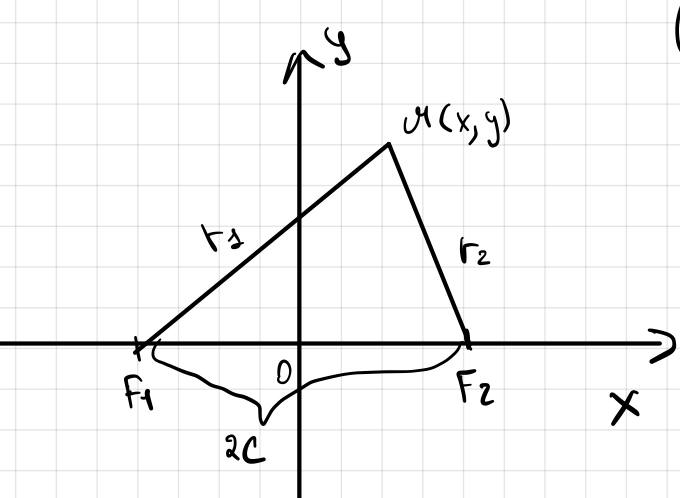
\includegraphics[width=0.5\linewidth]{images/Прямые 2 порядка/Гипербола/Гипербола.jpg}\\
\end{center}

\begin{equation}
	|r_1 - r_2| = 2a
\end{equation}

\begin{equation}
	|\sqrt{(x+c)^2+y^2} - \sqrt{(x - c)^2 + y^2}| = 2a
\end{equation}

\[x^2 + 2cy + c^2 + y^2 + x^2 - 2cx + c^2 + y^2 - 2\sqrt{(x^2 + 2cx + c^2 + y^2)(x^2 - 2cx + c^2 + y^2)} = 4a^2\]
\[ 2(x^2 + c^2 + y^2) - 2\sqrt{(x^2 + c^2 + y^2)^2 - 4c^2x^2} = 4a^2\]
\[ (x^2 + c^2 + y^2) = t^2\]
\[ t^2 - 2a^2 = \sqrt{t^4 - 4c^2x^2} \Rightarrow 4c^2x^2 - 4a^2(x^2 + c^2 + y^2) = -4a^4\]
\[ (c^2 - a^2)x^2 - a^2y^2 = a^2c^2 - a^4 = a^2(c^2-a^2) \]
\[ b^2x^2 - a^2y^2 = a^2b^2 \]
\begin{tcolorbox}
\begin{equation}
	\frac{x^2}{a^2} - \frac{y^2}{b^2} = 1
\end{equation}
\end{tcolorbox}

Проверим (3) $ \Rightarrow$ (1), (2)
\[ y^2 = (\frac{x^2}{a^2} - 1)b^2 \]
\[ r_1 = \sqrt{(x^2+c^2)+y^2} = \sqrt{x^2 + 2cx + c^2 + \frac{b^2}{a^2}x^2 - b^2} = \]
\[ b^2 = c^2 - a^2 \]
\[ \sqrt{x^2 + 2cx + c^2 + \frac{c^2}{a^2}x - \frac{a^2}{a^2}x^2 - c^2 + a^2} = \sqrt{a^2 + 2\frac{cx}{a}a + (\frac{cx}{a})^2} = \sqrt{(a+\frac{cx}{a})^2} = |a+\frac{cx}{a}| \]

\begin{tcolorbox}
	\[ r_1 = |a+\frac{cx}{a}| \]
	\[ r_2 = |a-\frac{cx}{a}| \]
\end{tcolorbox}

\begin{enumerate}
	\item $x > a$
	\[ r_1 = |a+\frac{cx}{a}| = a + \frac{cx}{a} \]
	\[ r_2 = |a-\frac{cx}{a}| = -a + \frac{cx}{a} \]
	\[ |r_1-r_2| = |a+\frac{cx}{a} + a - \frac{cx}{a}| = |2a| \]
	\item $x < -a$
	\[ |r_1-r_2| \]
	\[r_1 = |a + \frac{x}{a}c| = -a -\frac{x}{a}c\]
	\[ |\frac{x}{a}| > 0,\; c > x\; \frac{x}{a} < 0 \]
	\[r_2 = |a - \frac{c}{a}x| = a + \frac{c}{a}x\]
	\[ |r_1-r_2| = |-a-\frac{x}{a}c - a + \frac{c}{a}x|\]

\end{enumerate}

Введём $\hat{y_1} = \frac{b}{a}x$\\
Введём $\hat{y_2} = -\frac{b}{a}x$\\
Это будут уравнения диагоналей прямоугольника (асимптоты)
\[ y > 0, x\to +\infty \]
\[ y = \sqrt{(\frac{b^2}{a^2} - 1)b^2} \]



\[ y(x) - \hat{y_1}(x) = \sqrt{(\frac{x^2}{a^2}b^2)} - \frac{b}{a}x = \frac{\frac{x^2b^2}{a^2} - b^2 - \frac{b^2}{a^2}x^2}{\sqrt{\frac{x^2b^2}{a^2} - b^2} + \frac{b}{a}x} = \frac{-b^2}{\sqrt{\frac{b^2}{a^2} - b^2} \frac{b}{a}x } \xrightarrow[+\infty]{} 0 \]

\\a - действительная полуось\\
b - мнимая полуось\\
\begin{center}
	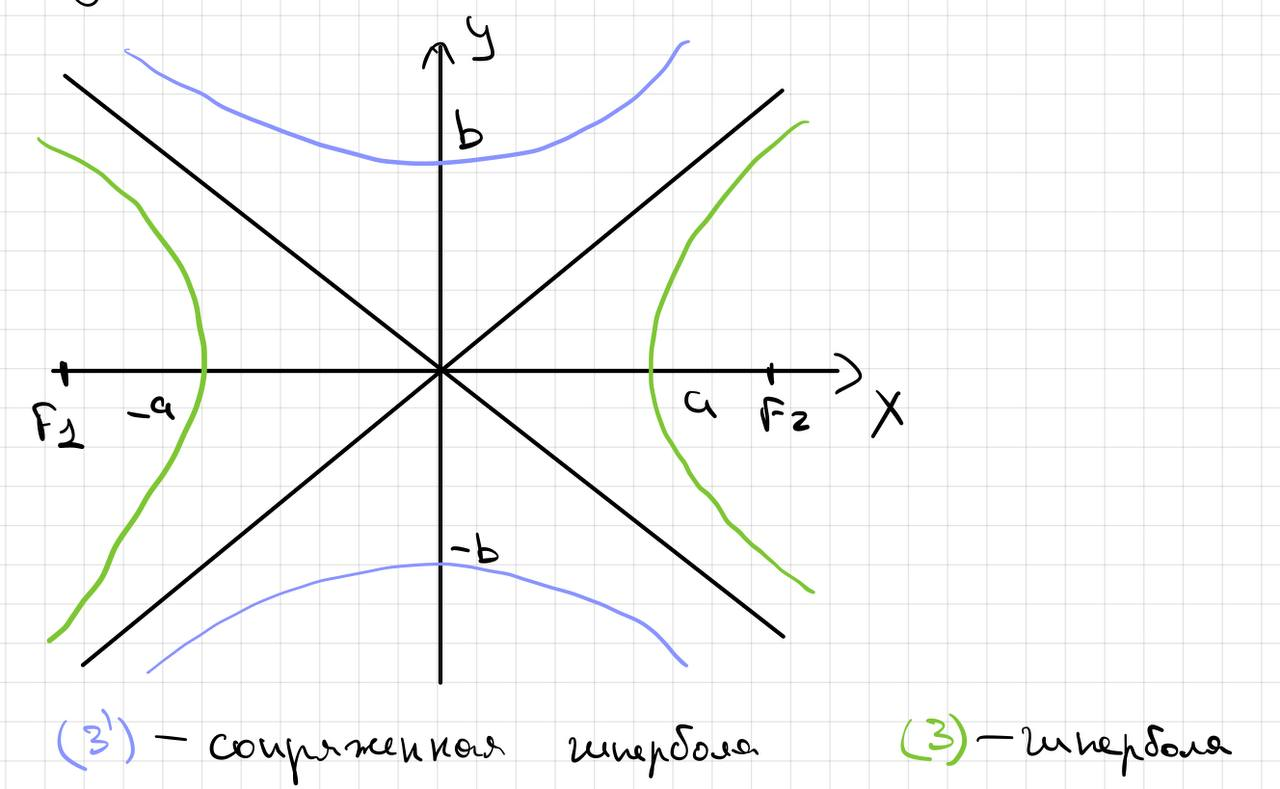
\includegraphics[width=0.5\linewidth]{images/Прямые 2 порядка/Гипербола/Прямоугольничек.jpg}\\
\end{center}
Свойства гиперболы:
\begin{enumerate}
	\item Симметрична относительно центра (начала координат)
	\item Фоуксы вне прямоугольника
	\item b и a никак не свДиректриса и екс/Директриса и екс.
\end{enumerate}

\subsection{Эксиетристет и директриса элипса и гиперболы.}
\textbf{Определение.} Эксиетристет это $e = \frac{c}{a}$\\
\begin{center}
	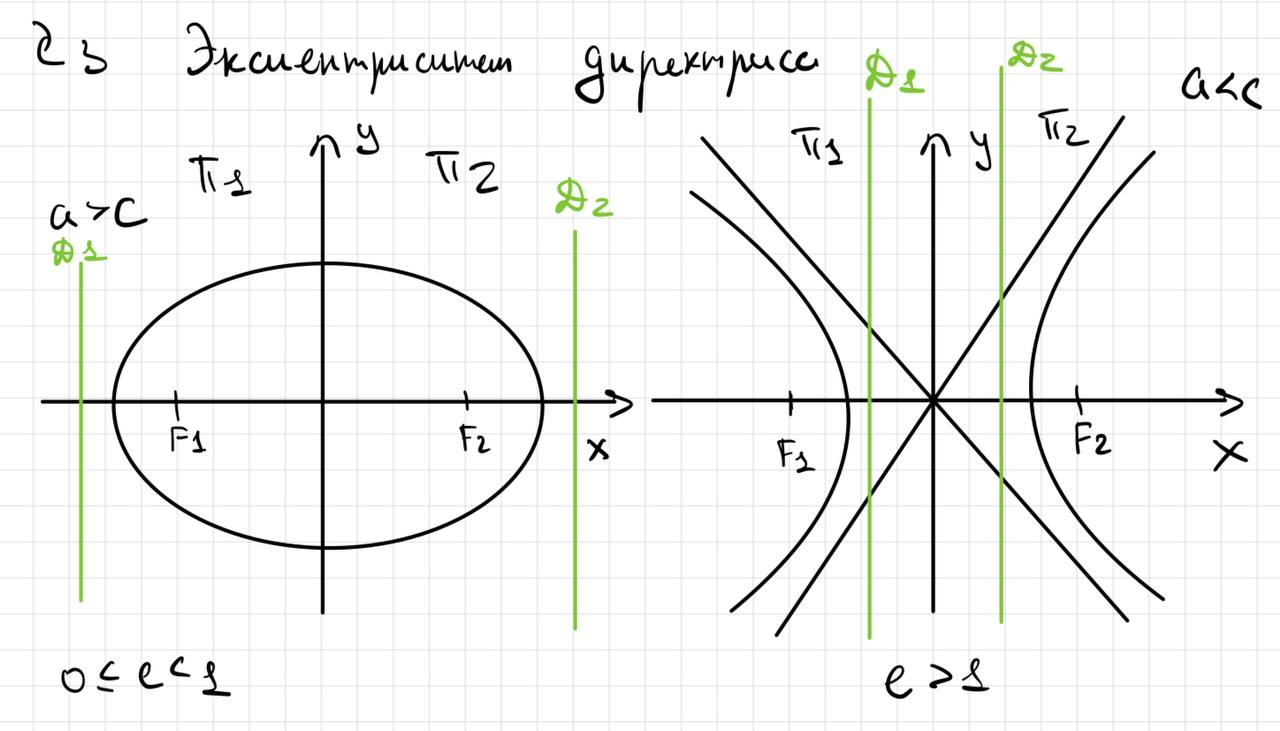
\includegraphics[width=0.5\linewidth]{images/Прямые 2 порядка/Директриса и екс/Директриса и екс.jpg}
\end{center}

Для элипса: $ 0 \leq e < 1$
Для окружности: $e=1$\\
Для гиперболы: $e > 1$
\[ 1 - e^2 = 1- \frac{c^2}{a^2} = \frac{a^2-c^2}{a^2} \]
Элипс: $1-e^2 = \frac{b^2}{a^2}$\\
Гипербола: $ e^2 - 1 = \frac{b^2}{a^2} $\\
\textbf{Определение.} Директрисы - это прямые ... в проебал
\[ \rho(D_i, 0) = \frac{a}{e} (or \frac{\pi}{e})  \]
\[D_1: -x=\frac{a}{e} \]
\[D_2: x=\frac{a}{e} \]
\begin{tcolorbox}
	\[-x - \frac{a}{e} = 0 \]
	\[x - \frac{a}{e} = 0 \]
\end{tcolorbox}
\textbf{Теорема. } $M(x, y)$\\
$r_i$ - ... радиусы = $\rho(M, F_1)$\\
$d_1 = \rhoM, D_i$
\[ \frac{r_i}{d_i} = e,\;\; i =1, 2 \]
\begin{tcolorbox}[title=Доказательство]
	\begin{enumerate}
		\item Элипс
		\[ r_1 = |a+\frac{c}{a}x| = a+\frac{c}{a}x = a + cx \]
		\[ d_1 = |-x -\frac{a}{e}| =  |x + \frac{a}{e}| = x+ \frac{a}{e} = \frac{ex+a}{e} \]
		\[ \frac{r_1}{d_1} = e \]
		\[ r_2 = |a-\frac{c}{a}x| = a-\frac{c}{a}x = a - cx \]
		\[ d_1 = |x -\frac{a}{e}| = -x + \frac{a}{e} = \frac{-ex+a}{e} \]
		\[ \frac{r_2}{d_2} = e \]
		Для элипса доказали. 
	\item Гипербола. Рассмотрим 1 случай, остальное по аналогии.\\
		\[ x \geq a, i=2 \]
		\[ r_2 = |a - \frac{c}{a}x| = -a + \frac{c}{a}x = -a + cx \]
		\[ d_2 = |x - \frac{a}{e}| = x - \frac{a}{e} = \frac{ex -a}{e} \]
		\[ \frac{r_2}{d_2} = e \]
		Доказали для гиперболы.
	\end{enumerate}
\end{tcolorbox}

\subsection{Парабола. Вывод канонического уравнения. Свойства параболы.}
\setcounter{equation}{0}
Парабола - множество точек плоскости таких что расстояние от которых до фиксированной точки плоскости (фокуса) равно расстоянию до фиксированной прямой (директрисы). \\
Фоукус на директрисе не лежит.\\

\begin{center}
	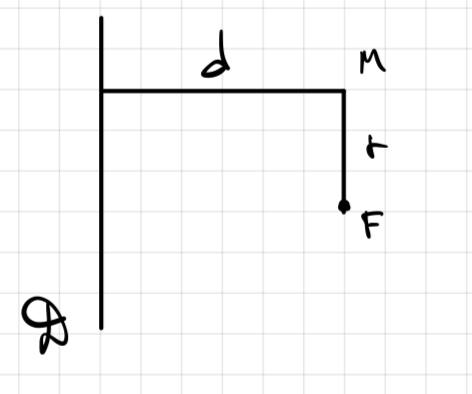
\includegraphics[width=0.4\linewidth]{images/Прямые 2 порядка/Парабола/Парабола 1.jpg}
	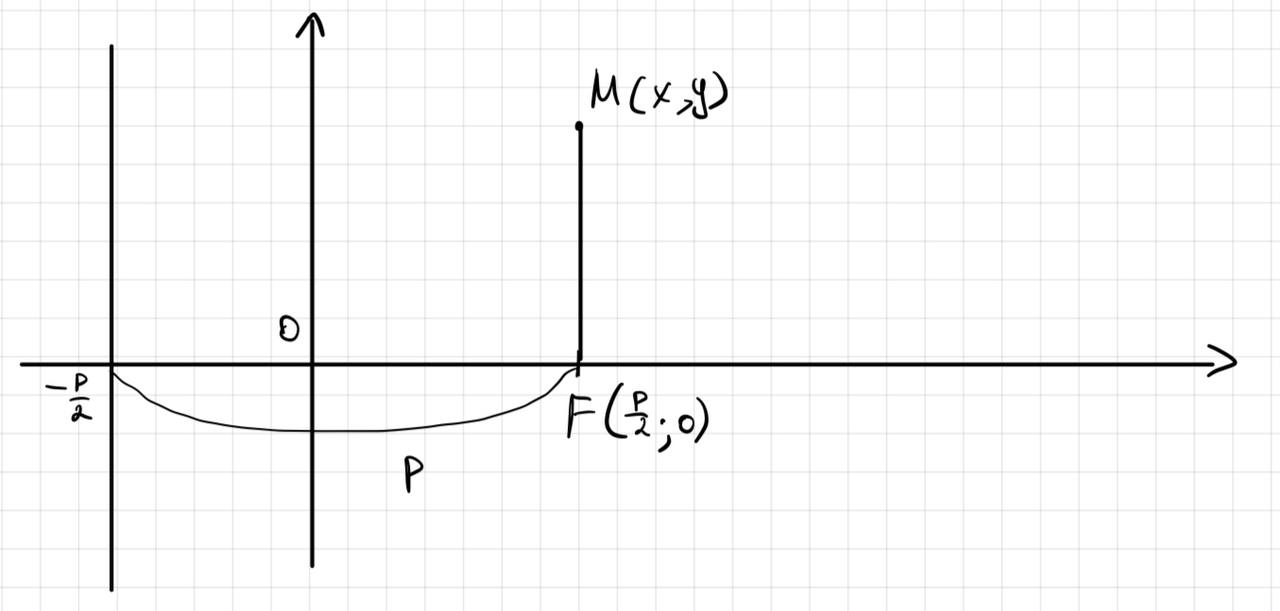
\includegraphics[width=0.55\linewidth]{images/Прямые 2 порядка/Парабола/Парабола 2.jpg}\\
\end{center}


\begin{equation}
	r = d
\end{equation}
Факальный параметр параболы: $P = \rho(F, D)$
$D: -x-\frac{P}{2} = 0$
\begin{equation}
	\sqrt{(x - \frac{P}{2})^2 + y^2} = |x + \frac{P}{2}| 
\end{equation}

\[ x^2 - px + \frac{p^2}{4} + y^2 = x^2 + px + \frac{p^2}{4} \]
Каноническое уравнение параболы:
\begin{equation}
	y^2 = 2px
\end{equation}

\begin{center}
	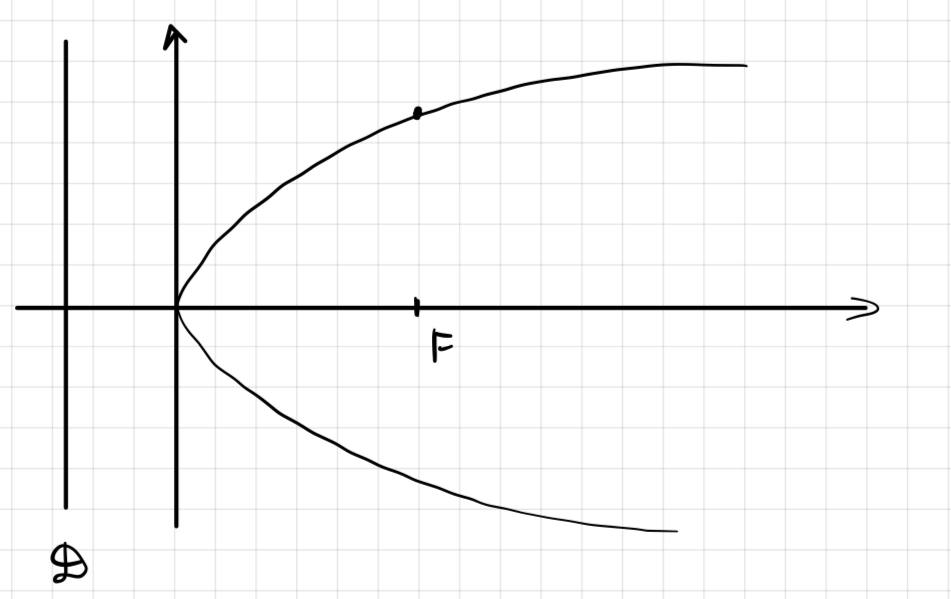
\includegraphics[width=0.5\linewidth]{images/Прямые 2 порядка/Парабола/Парабола 3.jpg}\\
\end{center}


Свойства параболы:
\begin{itemize}
	\item Симметрично относително Ox
	\item Расположено в правой полуплоскости (x > 0)
\end{itemize}

\subsection{Упрощение алгебраического уравнения второго порядка на плоскости. Преобразование коэфициентов уравнений второго порядка при ортогональных преобразованиях.}
\setcounter{equatoin}{0}
\subsubsection{Сдвиг.}
У нас есть ДПСК. $OXY \to O`X`Y`$\\
\[ A^2x^2 + 2B^2xy + Cy^2 + 2Dx + 2Ey + F = 0 \]
$A^2 + 2B^2xy + Cy^2$ - квадратная часть. ($A^2 + B^2 + C^2 > 0$)\\
$ 2Dx + 2Ey $ - линейная часть\\
$F$ - свободный член.

\begin{center}
	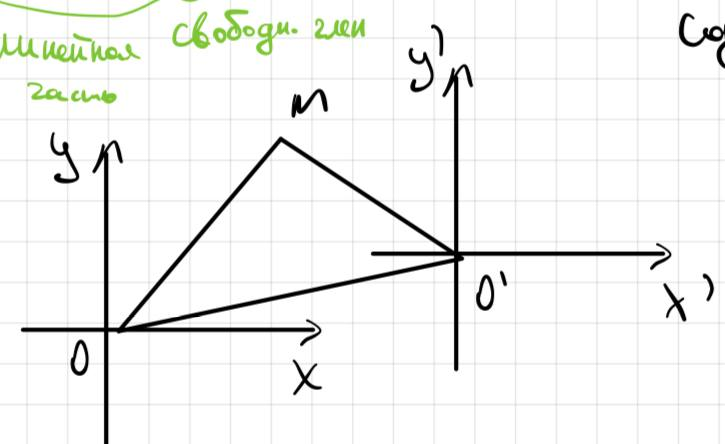
\includegraphics[width=0.5\linewidth]{images/Прямые 2 порядка/Преобразования алг коэф/Переход.jpg}\\
\end{center}


\[ 
	\begin{cases}
		x = x` + x_0\\
		y = y` + y_0\\
	\end{cases}
\]
\[ A`^2x`^2 + 2B^2`x`y` + C`y^2` + 2D`x` + 2E`y` + F` = 0 \]
\[ A(x^21 + 2x`x_0 + x_0` )  + 2B(x` + x_0) (y` + y_0) + C(y`^2 + 2y\psi_0 + y_0^2) + 2D(x`+ x_0) + 2E(y` + y_0) + F = 0 \]
$A` = A$, $D` = Ax_0 + By_0 + D$\\
$B`  B$, $C` = C$\\
$ F` = Ax_0^2 + 2Bx_0y_0 + Cy_0^2 + 2Dx_0 + 2Ey_0 + F $


















\end{document}
